\documentclass[xcolor=dvipsnames,12pt]{beamer}  % for hardcopy add 'trans'
\hypersetup{pdfpagemode=FullScreen}
\mode<presentation>
{
	\usecolortheme{seahorse}
	% Letras en negro para títulos 
	\setbeamercolor{title}{fg=royalazure}
	% Cambiar color de fondo de diapositivas y otros atributos
	\setbeamercolor{background canvas}{bg=whitesmoke}
	% -- Texto
	\setbeamercolor{normal text}{fg=black}
	% -- Título de diapositiva
	\setbeamercolor{frametitle}{fg=arsenic}
	% -- Bullet de itemize
	\setbeamercolor{item}{fg=cyan}
	% -- Texto
	\usebeamercolor[fg]{normal text}
	% -- Color de título de objeto flotante, como Figura o Tabla
	\setbeamercolor{caption name}{fg=magenta}
	
}

% Define some colors
\definecolor{whitesmoke}{rgb}{0.957, 0.957, 0.957}
\definecolor{arsenic}{rgb}{0.23, 0.27, 0.29}
\definecolor{charcoal}{rgb}{0.21, 0.27, 0.31}
\definecolor{royalazure}{rgb}{0.0, 0.22, 0.66}
\definecolor{rednsc}{rgb}{0.77, 0.01, 0.2}
\definecolor{raspberry}{rgb}{0.89, 0.04, 0.36}
% Fuente general 
\usepackage{fontawesome}
\usepackage{colortbl}
\usepackage{adjustbox}
\usefonttheme{professionalfonts}
\setbeamerfont{title}{series=\bfseries,parent=structure}
\setbeamerfont{frametitle}{series=\bfseries,parent=structure}
% Usaer fuente serif para matemáticas
\usefonttheme[onlymath]{serif}
% Para graficos
\usepackage{graphicx}
% Folder con gráficos
\graphicspath{{figs/}}

% Librerías para matemáticas
\usepackage{amsmath, amssymb, amsthm}
%\usepackage{kpfonts}
\usepackage{lmodern}

% Idioma
\usepackage[spanish,es-tabla]{babel}
\selectlanguage{spanish}
\decimalpoint
\usepackage[utf8]{inputenc}
% Para pies de tabla y de figura
\usepackage{caption}
% Contar figuras y tablas
\setbeamertemplate{caption}[numbered]

\usepackage{enumitem}
\setlist[itemize]{itemsep=10pt, label={\color{rednsc}\scriptsize \faCheckCircle}}


% tcolorbox 
\usepackage[most]{tcolorbox}
\usepackage{tikz}

\newtcolorbox{mybox}[2][]{%
	enhanced,
	colbacktitle=red!10!white,
	colback=blue!10!white,
	coltitle=raspberry!90!black,
	attach boxed title to top left={xshift=1cm,yshift=-\tcboxedtitleheight/2,yshifttext=-\tcboxedtitleheight/2},
	%attach boxed title to top center={yshift=-2mm},
	title={#2},
	drop fuzzy shadow southeast,%=black!50!white,
	fonttitle=\bfseries,
	#1
}

% para mostrar codigo
\usepackage{listings}

\lstset{ %
	language=R,                     % the language of the code
	basicstyle=\footnotesize\ttfamily\color{blue},       % the size of the fonts that are used for the code
	numbers=left,                   % where to put the line-numbers
	numberstyle=\tiny\color{gray},  % the style that is used for the line-numbers
	stepnumber=1,                   % the step between two line-numbers. If it's 1, each line
	% will be numbered
	numbersep=5pt,                  % how far the line-numbers are from the code
	% backgroundcolor=\color{black},  % choose the background color. You must add \usepackage{color}
	showspaces=false,               % show spaces adding particular underscores
	showstringspaces=false,         % underline spaces within strings
	showtabs=false,                 % show tabs within strings adding particular underscores
	frame=none,                   % adds a frame around the code
	rulecolor=\color{black},        % if not set, the frame-color may be changed on line-breaks within not-black text (e.g. commens (green here))
	tabsize=1,                      % sets default tabsize to 2 spaces
	captionpos=b,                   % sets the caption-position to bottom
	breaklines=true,                % sets automatic line breaking
	breakatwhitespace=false,        % sets if automatic breaks should only happen at whitespace
	title=\lstname,                 % show the filename of files included with \lstinputlisting;
	% also try caption instead of title
	keywordstyle=\color{RubineRed},      % keyword style
	commentstyle=\color{Green},   % comment style
	stringstyle=\color{RedOrange},      % string literal style
	% escapeinside={\%*}{*)},         % if you want to add a comment within your code
	morekeywords={*,\_, <-,...}            % if you want to add more keywords to the set
	% otherkeywords={!,!=,~,$,*,\&,\%/\%,\%*\%,\%\%,<-,<<-}
}

% Color of numbers inside lists
\lstset{literate=%
	{0}{{{\color{red}0}}}1
	{1}{{{\color{red}1}}}1
	{2}{{{\color{red}2}}}1
	{3}{{{\color{red}3}}}1
	{4}{{{\color{red}4}}}1
	{5}{{{\color{red}5}}}1
	{6}{{{\color{red}6}}}1
	{7}{{{\color{red}7}}}1
	{8}{{{\color{red}8}}}1
	{9}{{{\color{red}9}}}1
}

% monospace default color to red
\usepackage{xcolor}% http://ctan.org/pkg/xcolor
\let\oldtexttt\texttt% Store \texttt
\renewcommand{\texttt}[2][blue!90]{\textcolor{#1}{\ttfamily #2}}%

\renewcommand{\lstlistingname}{Código de R -}

% Plus symbol resized

\newcommand{\plus}{\raisebox{.1\height}{\scalebox{.5}{+}}}

% space in paragraphs
\usepackage{parskip}
% curly brackets in itemize
\usepackage{picture}
% Cambiar el espacio entre pie y figura
\setlength{\abovecaptionskip}{0pt plus 0pt minus 0pt}
\let\vec\mathbf
% Hacer itemize personalizado 
\newenvironment{myitemize}
{ \begin{itemize}
		\setlength{\itemsep}{1pt}
		\setlength{\parskip}{0pt}
		\setlength{\parsep}{0pt}   }
{ \end{itemize}                  } 

\title{{\sf Decisiones y teoría de juegos}}

\author{
	\textbf{Emmanuel Alcalá}
}

\date{\today}

\begin{document}
% Página de título
% Diapositiva 0
\begin{frame}
	\titlepage
	\tiny \LaTeXe\ %; {\color{RoyalBlue}\faRProject}
\end{frame}

% Diapositiva 1

\frame{
	\frametitle{Presentación}

	\textbf{¿Qué es la teoría de juegos?}

	\onslide<1->
	\begin{tcolorbox}[title=Definición: teoría de juegos, colframe=red!20!blue!70]

		Estudio y aplicación de los modelos matemáticos de interacción estratégica entre agentes racionales.

		La \textbf{teoría de juegos} provee un marco para la construcción de modelos que describen situaciones de conflicto y cooperación entre agentes \textit{racionales}.

	\end{tcolorbox}

	\onslide<2-> La \textbf{racionalidad} es entendida como la elección de acciones que \textit{maximizan} las ganancias sujeta a ciertas restricciones $\Rightarrow$ comportamiento racional.

	\onslide<3-> El \textbf{agente racional} es aquel que tiene preferencias definidas y modela su \textbf{incertidumbre} mediante una \textbf{función de utilidad }$U(\cdot)$ y \textit{optimiza} su utilidad sobre todas las posibles acciones.
}

\frame{
	\frametitle{Presentación}
	\onslide<1-> Por \textbf{agente} podemos entender personas u otras entidades, como empresas, gobiernos y otras instituciones (siempre de forma simplificada).

	\onslide<2-> Otra forma de definir la racionalidad del agente es que éste actúa de acuerdo a sus preferencias, asumiendo que sus preferencias están ordenadas (o tienen una \textit{ordenación débil}).

	\onslide<3-> En los problemas planteados en teoría de juegos, los agentes deben tener en cuenta lo que harán \textit{los otros agentes}.

}

\frame{
	\frametitle{Presentación}
	\onslide<1-> Podemos, en general, distinguir a los sistemas con agencia por su capacidad para adaptarse.

	\onslide<2-> A diferencia de los sistemas inertes y deterministas, los sistemas adaptables pueden responder de diferentes maneras según las circunstancias en su entorno, es decir, ajustan sus respuestas al ambiente (que incluye a otros agentes).

	\onslide<3-> A un sistema no adaptativo e inerte se le puede estudiar de forma aislada, a un sistema adaptativo con agencia no, dado que existe \textbf{interdependencia} entre este sistema y otros. $\Rightarrow$ no podemos predecir el comportamiento de un agente sin considerar el comportamiento del resto.

}

\frame{
	\frametitle{Nivel de agregación de los agentes}

	La teoría de juegos se puede aplicar en distintos niveles de agregación.

	Con \textbf{nivel de agregación} nos referimos entidades de jerarquía creciente, donde cada nivel $j$ está compuesto (es un \textit{agregado} de) de varios niveles $i$, a su vez es compositivo de nivel $k$.

	\begin{figure}
		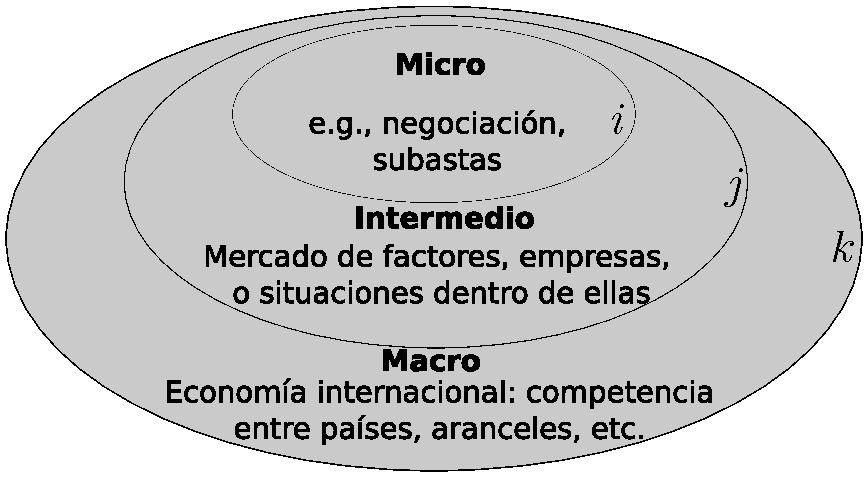
\includegraphics[scale=0.5]{agregacion}
	\end{figure}

}


\frame{
	\frametitle{Juegos vs decisiones individuales}

	\onslide<1-> Fernanda y Alejandra van a un bar.

	\onslide<2-> Fer escoge cerveza, Ale escoge mezcal.

	\onslide<3-> - Un problema de decisión individual.

	\onslide<4-> Fer y Ale deciden si dividir al cuenta.

	\onslide<5-> - Un juego (una interacción estratégica). Por ejemplo, Ale puede acceder a pagar toda la cuenta \textit{si} Fer paga el Uber, de otra forma, la cuenta será 50/50.

}

\frame{
	\frametitle{Ámbito de la teoría de juegos}
	Las acciones o decisiones pueden ser de dos tipos:

	\begin{itemize}
		\onslide<1-> \item Las que suceden en \textbf{contextos paramétricos}: la decisión del agente solo depende de los parámetros de una situación. Puede ocurrir en \textit{certidumbre} o \textit{incertidumbre}.
		      \onslide<2-> \item Las que suceden en \textbf{contextos estratégicos}: los resultados dependen de ciertos parámetros, \textit{y además} de las acciones de otros agentes. Existe una interacción estratégica cuando la acción del agente $i$ depende de sus expectativas sobre los demás agentes $-i$
	\end{itemize}
}


\frame{
	\frametitle{Ingredientes básicos de decisiones en contextos estratégicos}

	En resumen, la teoría de la elección racional, que revisaremos en la primera unidad, nos exige para nuestros agentes:

	\begin{itemize}
		\item Que tengan preferencias claras.
		\item Que se formen expectativas sobre lo que desconocen (i.e., decisiones bajo incertidumbre).
		\item Que tomen decisiones \textit{consistentes} con sus preferencias y expectativas.
	\end{itemize}
}

\frame{
	\frametitle{Modelos matemáticos}
	Incluso en niveles de agregación \textit{macro}, los modelos deben mantenerse lo más simples \textit{posibles}, pero no más simples.

	Un \textbf{modelo} es una idealización que simplifica un sistema, abstrayendo las relaciones necesarias y suficientes entre las variables, y dejando de lado aquellas menos relevantes.

	Un \textbf{modelo matemático} es una de estas idealizaciones, pero usando el lenguaje formal de las matemáticas.

	\begin{tcolorbox}[colback=Green!10]
		«Todo lo sencillo es falso. Todo lo complejo es inusable»
	\end{tcolorbox}
}

\frame{
	\frametitle{¿Para qué sirve teoría de juegos?}

	\onslide<1-> Antes de eso: ¿para qué sirve la educación universitaria?

	\onslide<2->
	\begin{tcolorbox}[colback=red!10]

		``Tenemos que darnos cuenta que vivimos en una cultura de consumidores... No hay participación activa productiva, una realización significativa de respuestas importantes a la vida. Entonces ¿qué esperamos de nuestra generación joven?"

		\onslide<3-> ``Desde el principio, el ITESO no se contenta con ser un \textit{simple conjunto de carreras, ni se interesa solamente en preparar técnicos o profesionales}, por cualificados que sean. Por el contrario, el ITESO intenta ser ante todo una \textbf{universidad}".
	\end{tcolorbox}

}

\frame{

	\onslide<1-> ¿Qué es una Universidad?

	\begin{itemize}
		\item \onslide<2-> ``...el conjunto de todas las cosas"

		\item \onslide<3-> ``Entendida la Universidad como generadora del saber, se le atribuyó el carácter de 'Alma Mater' en el sentido de engendrar y transformar al hombre por obra de la ciencia y el saber."

		\item \onslide<4-> ``El ITESO intenta ser ante todo una universidad: el lugar en que confluyen todos los miembros de la comunidad para la búsqueda de la verdad, para la creación y transmisión de la cultura"
	\end{itemize}
}

\frame{
	\frametitle{¿Para qué sirve teoría de juegos?}

	\textbf{Mi respuesta:} para responder a preguntas como

	\onslide<2->
	\begin{myitemize}
		\item ¿Qué decisiones tomar cuando mis ganancias dependen de lo que haga otra persona?
		\item ¿Cómo anticiparme a las decisiones de alguien más si el resultado puede afectarme?
		\item ¿Cómo debo tomar elecciones cuando hay algo que no conozco sobre la situación?
	\end{myitemize}

	\onslide<3-> Pero, más importante, puede ayudarnos a entender cuestiones más trascendentales...

}

\frame{
	\textbf{¡Por qué carajo nadie le hizo caso a los científicos de \textit{Don't look up}...}

	\onslide<2->
	\begin{figure}
		\centering
		
\includegraphics[width=0.6\linewidth]{debiasky_rant.png}
	\end{figure}
}

\frame{

	Resulta que tenemos un caso similar, ejemplificado por el cambio climático

	\begin{figure}
		\centering
		\onslide<2->
		\begin{minipage}{0.5\textwidth}
			\centering
			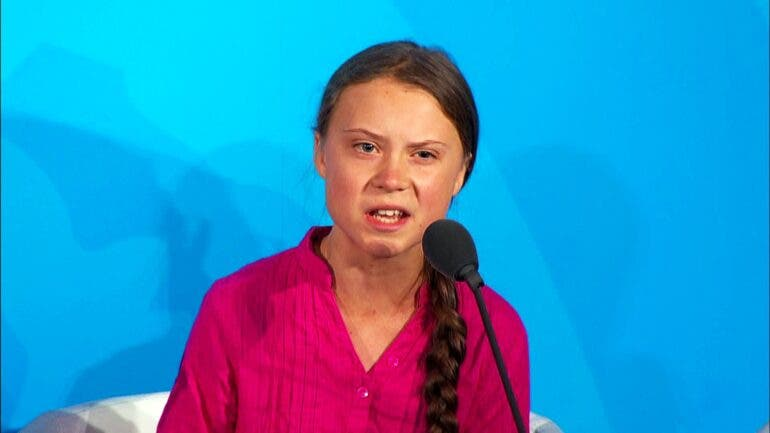
\includegraphics[width=0.9\textwidth]{greta.jpeg} % first figure itself
		\end{minipage}\hfill\onslide<3->
		\begin{minipage}{0.5\textwidth}
			\centering
			
\includegraphics[width=0.9\textwidth]{trum_mockery.png} % second figure itself
		\end{minipage}
		\caption*{“How dare you?”}
	\end{figure}

	\onslide<3-> La pregunta es, por supuesto, ¿por qué no se han tomado acciones contundentes? Se sabe desde los 70s, solo que ahora estamos \textit{casi} 100\% seguros.

}

\frame{
	\textbf{Perspectiva desde Teoría de Juegos}

	\onslide<2-> La mitigación del cambio climático es un problema de \textit{\textbf{bien común global}}: a nivel individual y de país, existen costos privados por la mitigación, pero el beneficio es compartido \textit{globalmente}, independientemente de la contribución de la persona/país.

	\onslide<5-> Lo anterior da origen a un problema que, según la \textit{economía experimental}, reduce la conducta prosocial o cooperativa en los humanos: el \textbf{problema del polizón o consumidor parásito} (\textit{free-rider}). Un polizón tiene \textit{\textbf{incentivos}} para no compartir equitativamente el costo de un bien, pero sí disfrutar de él. Esto eventualmente degrada al bien o, incluso, impide que suceda.

}


\frame{
	\frametitle{Objetivos del curso}
	\textbf{Libros}

	\begin{minipage}{\linewidth}
		\centering
		\begin{minipage}{0.42\linewidth}
			\begin{figure}[H]
				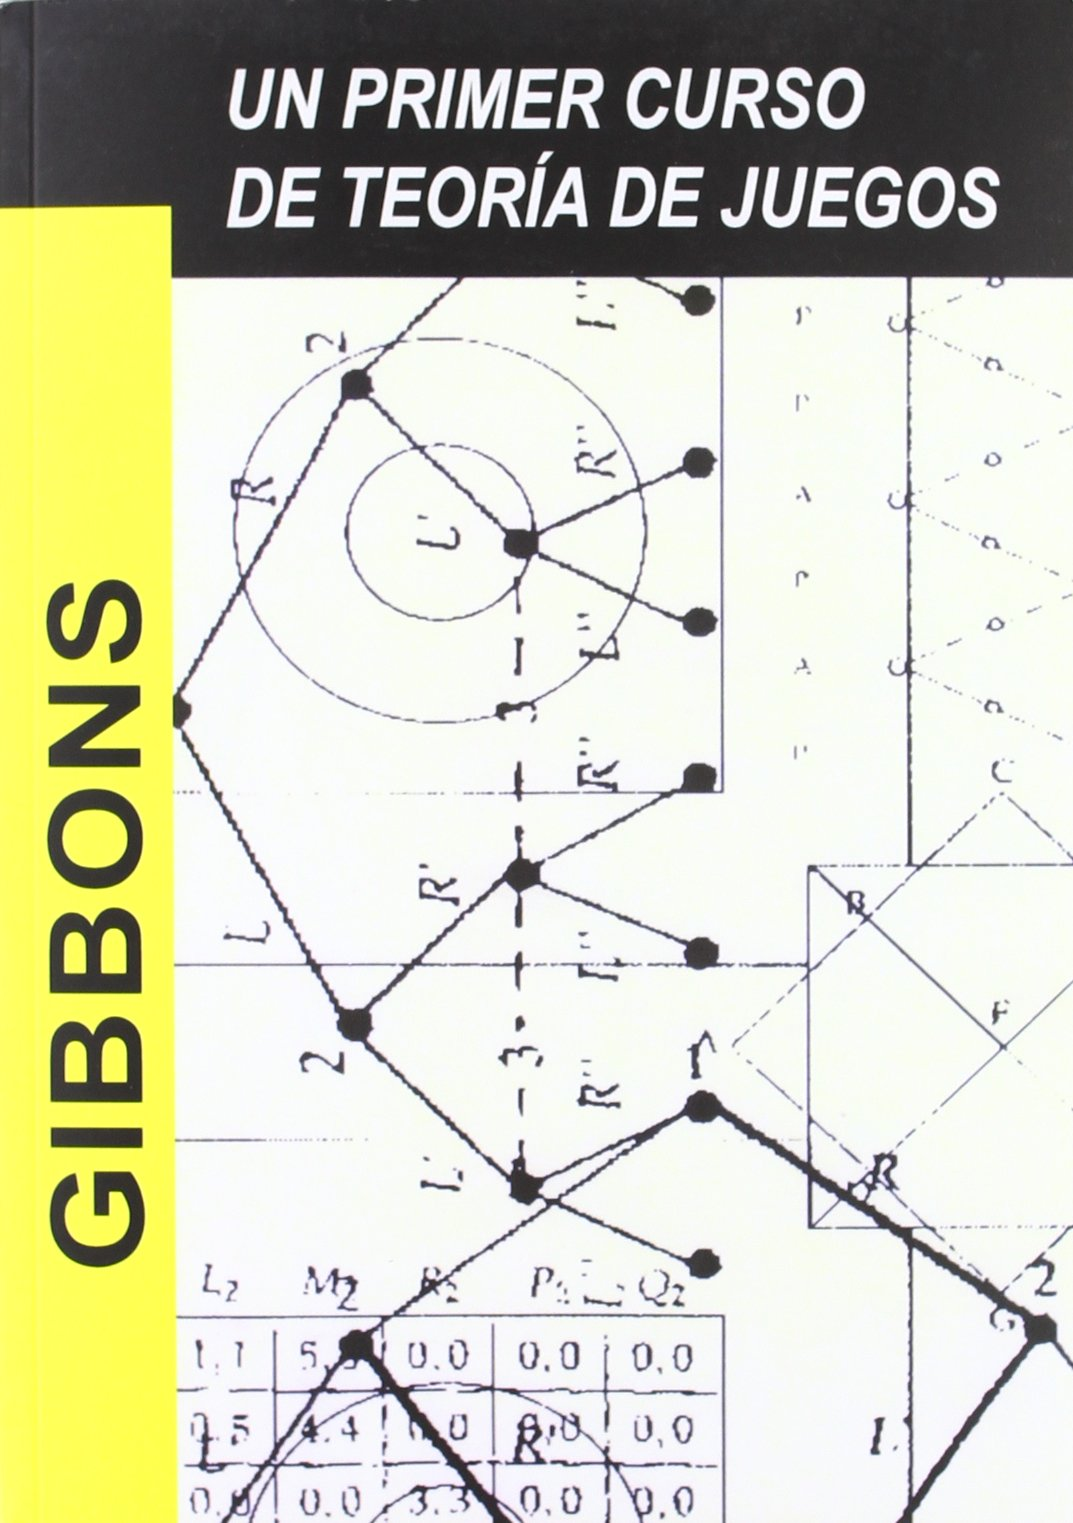
\includegraphics[width=0.9\textwidth]{gibbons_book.png}
			\end{figure}
		\end{minipage}
		\hspace{0.05\linewidth}
		\begin{minipage}{0.42\linewidth}
			\begin{figure}[H]
				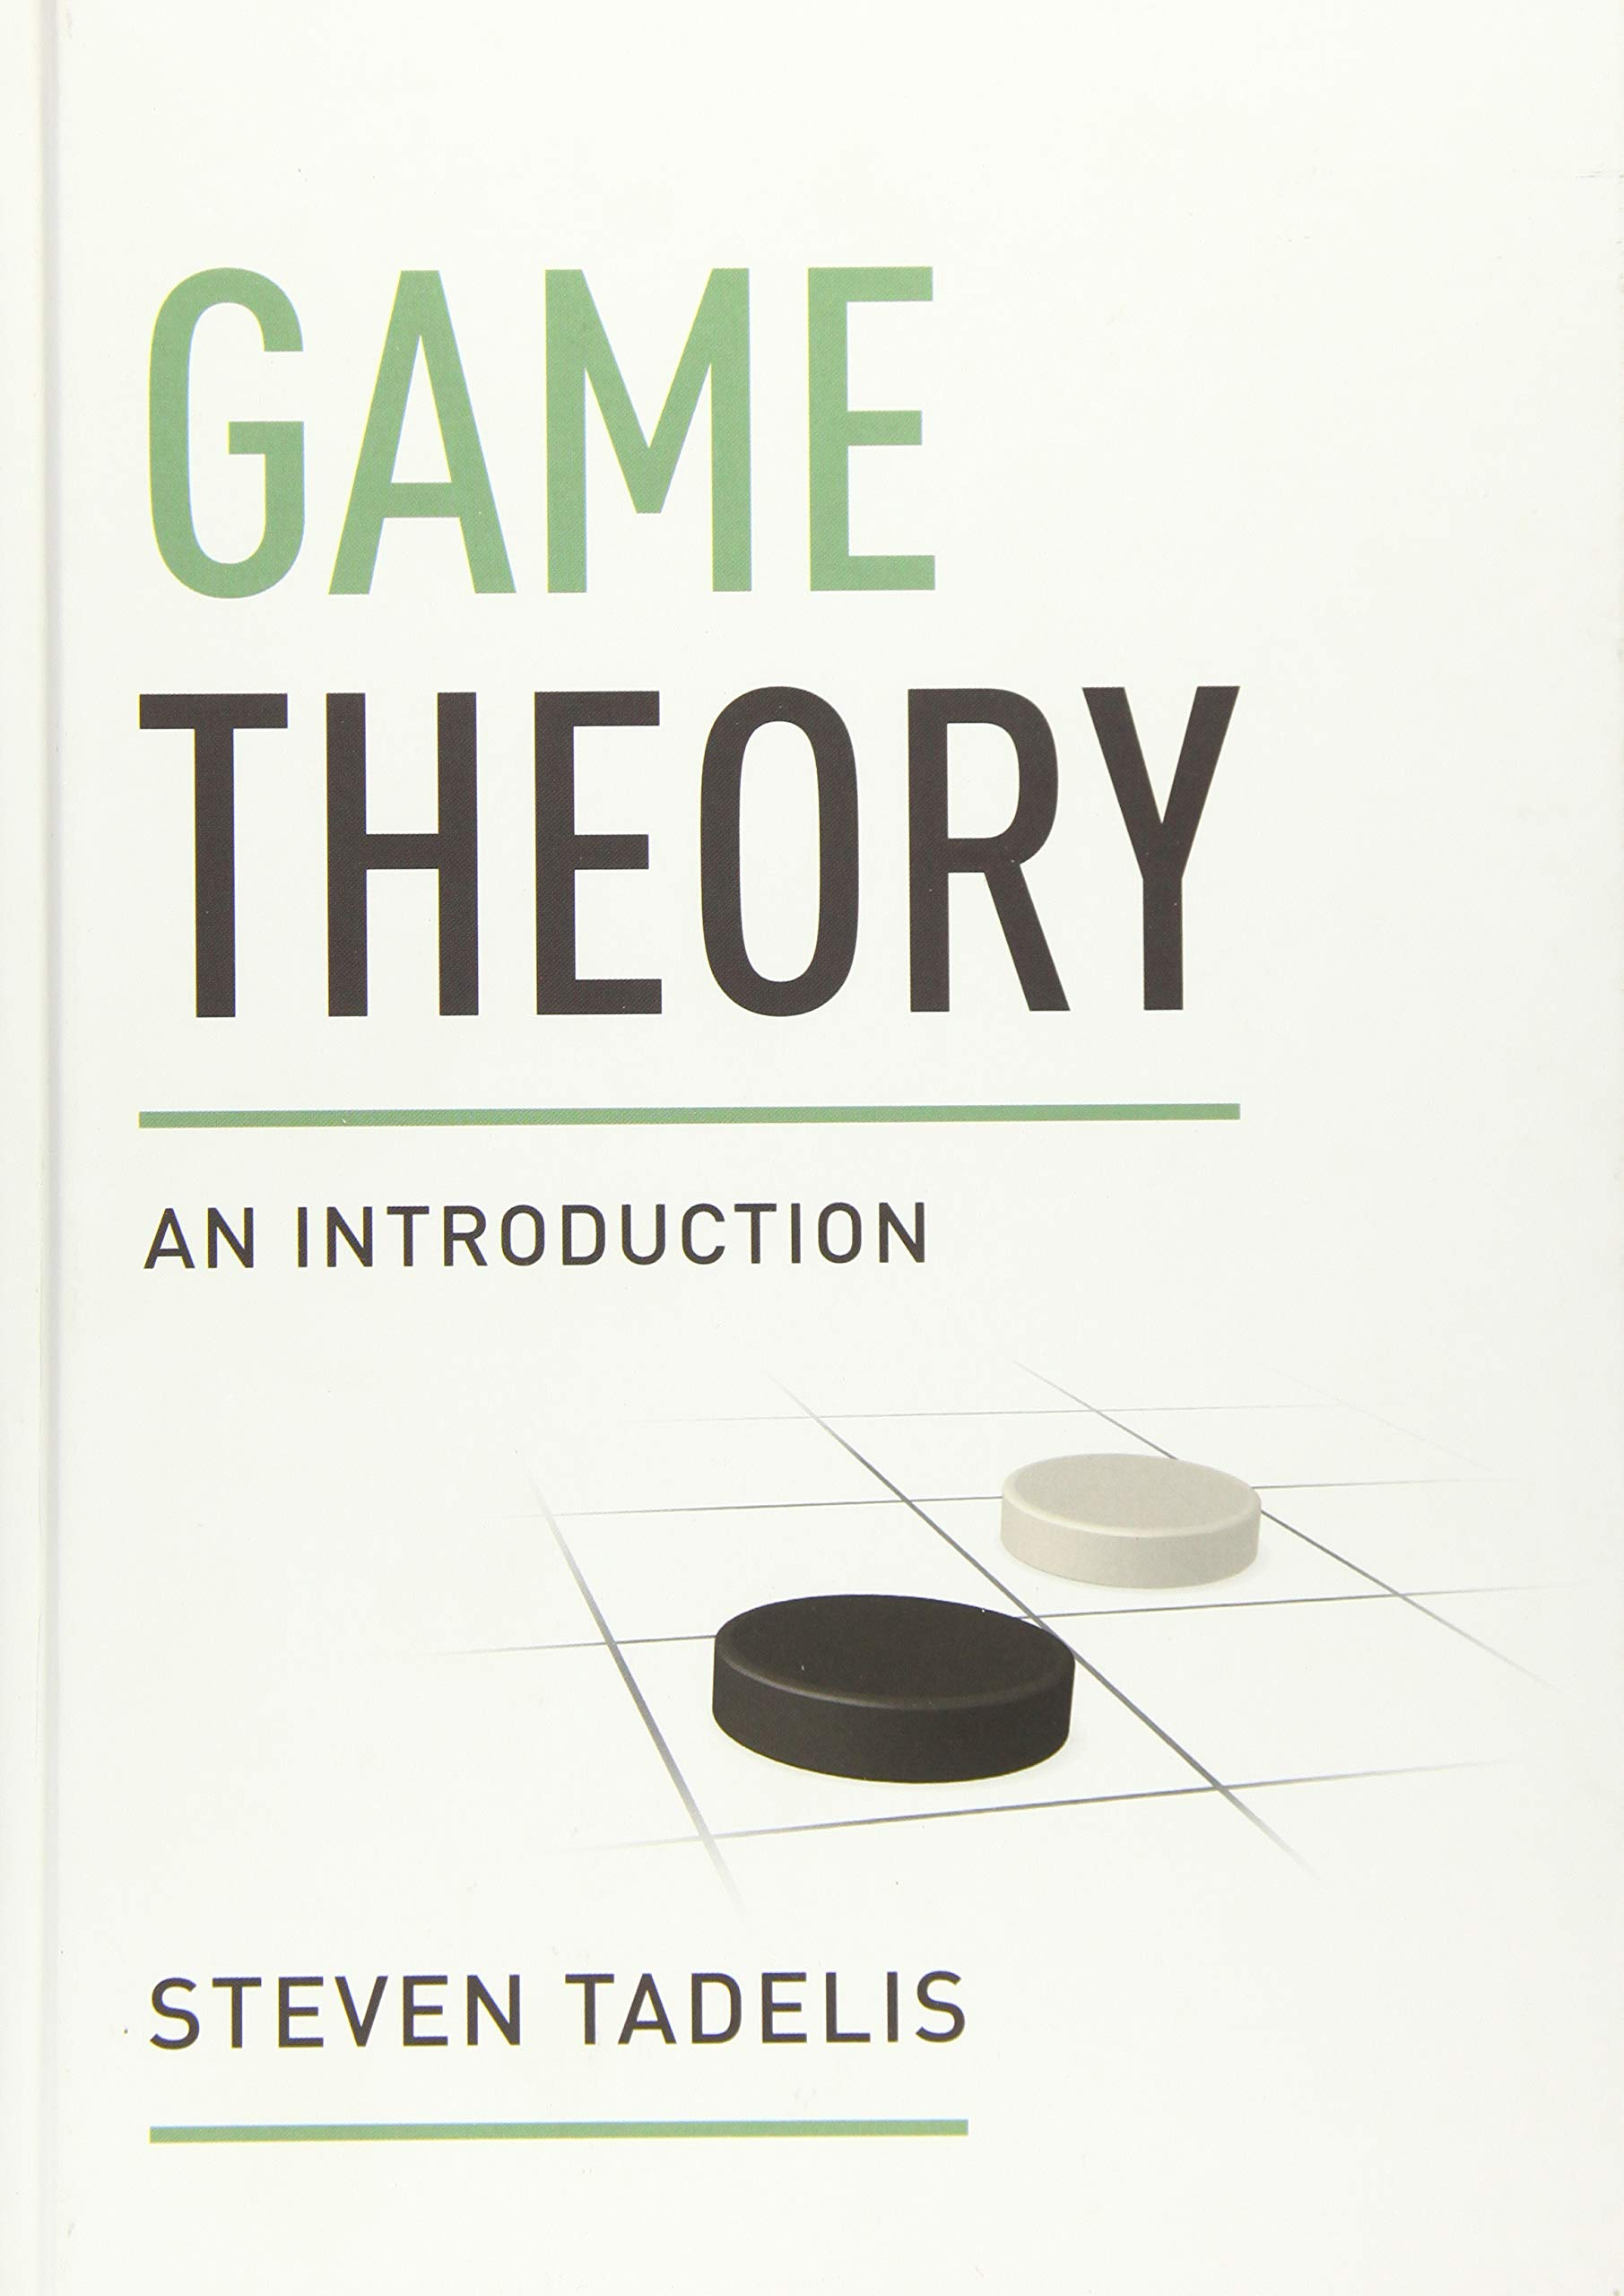
\includegraphics[width=0.9\textwidth]{tadelis.png}
			\end{figure}
		\end{minipage}
	\end{minipage}

}
\frame{
	\frametitle{Objetivos del curso}
	\begin{enumerate}
		\item \textbf{Tema 1}: Teoría de la utilidad esperada \\
		      \textit{Tadelis, cáps. 1-3}.\\
		      \textbf{Tema 2}: Juegos estáticos con información completa.\\
		      \textit{Gibbons, cáp. 1; Tadelis, cáps. 3-6}.
		\item \textbf{Tema único}: Juegos dinámicos con información completa\\
		      \textit{Gibbons, cáp. 2; Tadelis, cáps. 7-11}.
		\item \textbf{Tema único}: Juegos estáticos con información incompleta\\
		      \textit{Gibbons, cáp. 3; Tadelis, cáps. 12-14}.
		\item \textbf{Tema único}: Juegos dinámicos con información incompleta.\\
		      \textit{Gibbons, cáp. 4; Tadelis, cáps. 15-18}.
	\end{enumerate}

	% 		{\color{BlueGreen} \textbf{CANVAS $\rightarrow$ Archivos $\rightarrow$ Referencias}}
}

\frame{
	\frametitle{Evaluación}

	\begin{table}[ht]
		\centering
		\begin{tabular}{|l@{\hspace{4em}}|l|}
			\hline
			\rowcolor{gray!25}
			\multicolumn{2}{|c|}{\textbf{Evaluación de calificación}} \\ \hline
			\bf Productos  & \bf  \% de la calificación               \\
			Exámenes       & 60 \%                                    \\
			Tareas         & 40 \%                                    \\
			Proyecto final & 0 \%                                     \\
			\hline
			\textbf{Total} & 100\%                                    \\
			\hline
		\end{tabular}
	\end{table}% 

	Tareas: una por unidad, cada una con valor de 10 pts. \\
	Eventualmente podré dejar ejercicios para puntos extra. \\
	\textbf{Copiar o plagiar tareas y exámenes será sancionado}.
}

\frame{
	\frametitle{Otros aspectos del curso}

	\onslide<2-> 1. Habrá una página de Github para el curso donde colocaré las notas del curso, las tareas y sus soluciones, y las ligas a los videos de Zoom (siempre que aplique).

		{\footnotesize \color{red}\url{https://jealcalat.github.io/Decisiones_Teoria_Juegos/}}

	\onslide<3-> 2. Las fechas de los exámenes, así como el formato de su aplicación (e.g., en línea vs en físico), serán determinadas durante la primera semana, y puestas públicamente en la página de CANVAS.

	\onslide<4-> 3. Al final del semestre podrán obtener puntos extra. La forma de hacerlo se explica en la página \textbf{Trabajo Extra} en CANVAS.

	\onslide<5-> 4. Las clases serán dictadas \textit{a mano}, por lo que requieren escribir para tomar sus propias notas. Las notas que yo proveeré estarán incompletas.
}

\frame{
	\onslide<1-> 5. Asesorías: previa cita por correo. Para agendar una cita, asegurarse de lo siguiente:
	\begin{itemize}
		\setlength{\itemsep}{0pt}
		\setlength{\parskip}{0pt}
		\setlength{\parsep}{0pt}
		\item Haber leído las notas de clase.
		\item Haber consultado los libros de texto del curso.
		\item Haber repasado, si está disponible, la grabación de la clase.
	\end{itemize}
}

\end{document}